% Created by tikzDevice version 0.12 on 2019-02-08 11:01:06
% !TEX encoding = UTF-8 Unicode
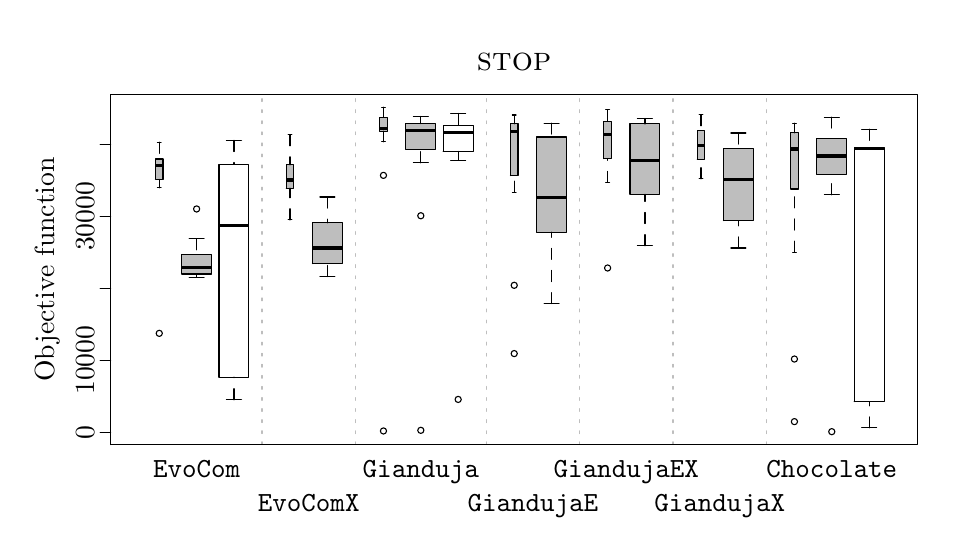
\begin{tikzpicture}[x=1pt,y=1pt]
\definecolor{fillColor}{RGB}{255,255,255}
\path[use as bounding box,fill=fillColor,fill opacity=0.00] (0,0) rectangle (325.21,180.67);
\begin{scope}
\path[clip] ( 30.00, 30.00) rectangle (321.61,156.67);
\definecolor{fillColor}{RGB}{190,190,190}

\path[fill=fillColor] ( 46.20,125.83) --
	( 48.90,125.83) --
	( 48.90,133.22) --
	( 46.20,133.22) --
	cycle;
\definecolor{drawColor}{RGB}{0,0,0}

\path[draw=drawColor,line width= 1.2pt,line join=round] ( 46.20,130.81) -- ( 48.90,130.81);

\path[draw=drawColor,line width= 0.4pt,dash pattern=on 4pt off 4pt ,line join=round,line cap=round] ( 47.55,122.81) -- ( 47.55,125.83);

\path[draw=drawColor,line width= 0.4pt,dash pattern=on 4pt off 4pt ,line join=round,line cap=round] ( 47.55,139.29) -- ( 47.55,133.22);

\path[draw=drawColor,line width= 0.4pt,line join=round,line cap=round] ( 46.88,122.81) -- ( 48.23,122.81);

\path[draw=drawColor,line width= 0.4pt,line join=round,line cap=round] ( 46.88,139.29) -- ( 48.23,139.29);

\path[draw=drawColor,line width= 0.4pt,line join=round,line cap=round] ( 46.20,125.83) --
	( 48.90,125.83) --
	( 48.90,133.22) --
	( 46.20,133.22) --
	( 46.20,125.83);

\path[draw=drawColor,line width= 0.4pt,line join=round,line cap=round] ( 47.55, 70.21) circle (  1.12);

\path[fill=fillColor] ( 55.65, 91.67) --
	( 66.45, 91.67) --
	( 66.45, 98.55) --
	( 55.65, 98.55) --
	cycle;

\path[draw=drawColor,line width= 1.2pt,line join=round] ( 55.65, 93.93) -- ( 66.45, 93.93);

\path[draw=drawColor,line width= 0.4pt,dash pattern=on 4pt off 4pt ,line join=round,line cap=round] ( 61.05, 90.45) -- ( 61.05, 91.67);

\path[draw=drawColor,line width= 0.4pt,dash pattern=on 4pt off 4pt ,line join=round,line cap=round] ( 61.05,104.35) -- ( 61.05, 98.55);

\path[draw=drawColor,line width= 0.4pt,line join=round,line cap=round] ( 58.35, 90.45) -- ( 63.75, 90.45);

\path[draw=drawColor,line width= 0.4pt,line join=round,line cap=round] ( 58.35,104.35) -- ( 63.75,104.35);

\path[draw=drawColor,line width= 0.4pt,line join=round,line cap=round] ( 55.65, 91.67) --
	( 66.45, 91.67) --
	( 66.45, 98.55) --
	( 55.65, 98.55) --
	( 55.65, 91.67);

\path[draw=drawColor,line width= 0.4pt,line join=round,line cap=round] ( 61.05,115.16) circle (  1.12);
\definecolor{fillColor}{RGB}{255,255,255}

\path[fill=fillColor] ( 69.15, 54.36) --
	( 79.95, 54.36) --
	( 79.95,131.37) --
	( 69.15,131.37) --
	cycle;

\path[draw=drawColor,line width= 1.2pt,line join=round] ( 69.15,109.09) -- ( 79.95,109.09);

\path[draw=drawColor,line width= 0.4pt,dash pattern=on 4pt off 4pt ,line join=round,line cap=round] ( 74.55, 46.19) -- ( 74.55, 54.36);

\path[draw=drawColor,line width= 0.4pt,dash pattern=on 4pt off 4pt ,line join=round,line cap=round] ( 74.55,139.93) -- ( 74.55,131.37);

\path[draw=drawColor,line width= 0.4pt,line join=round,line cap=round] ( 71.85, 46.19) -- ( 77.25, 46.19);

\path[draw=drawColor,line width= 0.4pt,line join=round,line cap=round] ( 71.85,139.93) -- ( 77.25,139.93);

\path[draw=drawColor,line width= 0.4pt,line join=round,line cap=round] ( 69.15, 54.36) --
	( 79.95, 54.36) --
	( 79.95,131.37) --
	( 69.15,131.37) --
	( 69.15, 54.36);
\definecolor{fillColor}{RGB}{190,190,190}

\path[fill=fillColor] ( 93.45,122.67) --
	( 96.15,122.67) --
	( 96.15,131.13) --
	( 93.45,131.13) --
	cycle;

\path[draw=drawColor,line width= 1.2pt,line join=round] ( 93.45,125.60) -- ( 96.15,125.60);

\path[draw=drawColor,line width= 0.4pt,dash pattern=on 4pt off 4pt ,line join=round,line cap=round] ( 94.80,111.22) -- ( 94.80,122.67);

\path[draw=drawColor,line width= 0.4pt,dash pattern=on 4pt off 4pt ,line join=round,line cap=round] ( 94.80,142.00) -- ( 94.80,131.13);

\path[draw=drawColor,line width= 0.4pt,line join=round,line cap=round] ( 94.13,111.22) -- ( 95.48,111.22);

\path[draw=drawColor,line width= 0.4pt,line join=round,line cap=round] ( 94.13,142.00) -- ( 95.48,142.00);

\path[draw=drawColor,line width= 0.4pt,line join=round,line cap=round] ( 93.45,122.67) --
	( 96.15,122.67) --
	( 96.15,131.13) --
	( 93.45,131.13) --
	( 93.45,122.67);

\path[fill=fillColor] (102.90, 95.42) --
	(113.70, 95.42) --
	(113.70,110.17) --
	(102.90,110.17) --
	cycle;

\path[draw=drawColor,line width= 1.2pt,line join=round] (102.90,101.08) -- (113.70,101.08);

\path[draw=drawColor,line width= 0.4pt,dash pattern=on 4pt off 4pt ,line join=round,line cap=round] (108.30, 90.72) -- (108.30, 95.42);

\path[draw=drawColor,line width= 0.4pt,dash pattern=on 4pt off 4pt ,line join=round,line cap=round] (108.30,119.49) -- (108.30,110.17);

\path[draw=drawColor,line width= 0.4pt,line join=round,line cap=round] (105.60, 90.72) -- (111.00, 90.72);

\path[draw=drawColor,line width= 0.4pt,line join=round,line cap=round] (105.60,119.49) -- (111.00,119.49);

\path[draw=drawColor,line width= 0.4pt,line join=round,line cap=round] (102.90, 95.42) --
	(113.70, 95.42) --
	(113.70,110.17) --
	(102.90,110.17) --
	(102.90, 95.42);

\path[fill=fillColor] (127.20,143.24) --
	(129.91,143.24) --
	(129.91,148.37) --
	(127.20,148.37) --
	cycle;

\path[draw=drawColor,line width= 1.2pt,line join=round] (127.20,144.30) -- (129.91,144.30);

\path[draw=drawColor,line width= 0.4pt,dash pattern=on 4pt off 4pt ,line join=round,line cap=round] (128.56,139.41) -- (128.56,143.24);

\path[draw=drawColor,line width= 0.4pt,dash pattern=on 4pt off 4pt ,line join=round,line cap=round] (128.56,151.98) -- (128.56,148.37);

\path[draw=drawColor,line width= 0.4pt,line join=round,line cap=round] (127.88,139.41) -- (129.23,139.41);

\path[draw=drawColor,line width= 0.4pt,line join=round,line cap=round] (127.88,151.98) -- (129.23,151.98);

\path[draw=drawColor,line width= 0.4pt,line join=round,line cap=round] (127.20,143.24) --
	(129.91,143.24) --
	(129.91,148.37) --
	(127.20,148.37) --
	(127.20,143.24);

\path[draw=drawColor,line width= 0.4pt,line join=round,line cap=round] (128.56,127.30) circle (  1.12);

\path[draw=drawColor,line width= 0.4pt,line join=round,line cap=round] (128.56, 34.94) circle (  1.12);

\path[fill=fillColor] (136.66,136.70) --
	(147.46,136.70) --
	(147.46,146.01) --
	(136.66,146.01) --
	cycle;

\path[draw=drawColor,line width= 1.2pt,line join=round] (136.66,143.41) -- (147.46,143.41);

\path[draw=drawColor,line width= 0.4pt,dash pattern=on 4pt off 4pt ,line join=round,line cap=round] (142.06,131.84) -- (142.06,136.70);

\path[draw=drawColor,line width= 0.4pt,dash pattern=on 4pt off 4pt ,line join=round,line cap=round] (142.06,148.57) -- (142.06,146.01);

\path[draw=drawColor,line width= 0.4pt,line join=round,line cap=round] (139.36,131.84) -- (144.76,131.84);

\path[draw=drawColor,line width= 0.4pt,line join=round,line cap=round] (139.36,148.57) -- (144.76,148.57);

\path[draw=drawColor,line width= 0.4pt,line join=round,line cap=round] (136.66,136.70) --
	(147.46,136.70) --
	(147.46,146.01) --
	(136.66,146.01) --
	(136.66,136.70);

\path[draw=drawColor,line width= 0.4pt,line join=round,line cap=round] (142.06,112.71) circle (  1.12);

\path[draw=drawColor,line width= 0.4pt,line join=round,line cap=round] (142.06, 35.17) circle (  1.12);
\definecolor{fillColor}{RGB}{255,255,255}

\path[fill=fillColor] (150.16,135.99) --
	(160.96,135.99) --
	(160.96,145.30) --
	(150.16,145.30) --
	cycle;

\path[draw=drawColor,line width= 1.2pt,line join=round] (150.16,142.86) -- (160.96,142.86);

\path[draw=drawColor,line width= 0.4pt,dash pattern=on 4pt off 4pt ,line join=round,line cap=round] (155.56,132.77) -- (155.56,135.99);

\path[draw=drawColor,line width= 0.4pt,dash pattern=on 4pt off 4pt ,line join=round,line cap=round] (155.56,149.64) -- (155.56,145.30);

\path[draw=drawColor,line width= 0.4pt,line join=round,line cap=round] (152.86,132.77) -- (158.26,132.77);

\path[draw=drawColor,line width= 0.4pt,line join=round,line cap=round] (152.86,149.64) -- (158.26,149.64);

\path[draw=drawColor,line width= 0.4pt,line join=round,line cap=round] (150.16,135.99) --
	(160.96,135.99) --
	(160.96,145.30) --
	(150.16,145.30) --
	(150.16,135.99);

\path[draw=drawColor,line width= 0.4pt,line join=round,line cap=round] (155.56, 46.34) circle (  1.12);
\definecolor{fillColor}{RGB}{190,190,190}

\path[fill=fillColor] (174.46,127.22) --
	(177.16,127.22) --
	(177.16,145.88) --
	(174.46,145.88) --
	cycle;

\path[draw=drawColor,line width= 1.2pt,line join=round] (174.46,143.09) -- (177.16,143.09);

\path[draw=drawColor,line width= 0.4pt,dash pattern=on 4pt off 4pt ,line join=round,line cap=round] (175.81,121.22) -- (175.81,127.22);

\path[draw=drawColor,line width= 0.4pt,dash pattern=on 4pt off 4pt ,line join=round,line cap=round] (175.81,149.11) -- (175.81,145.88);

\path[draw=drawColor,line width= 0.4pt,line join=round,line cap=round] (175.13,121.22) -- (176.48,121.22);

\path[draw=drawColor,line width= 0.4pt,line join=round,line cap=round] (175.13,149.11) -- (176.48,149.11);

\path[draw=drawColor,line width= 0.4pt,line join=round,line cap=round] (174.46,127.22) --
	(177.16,127.22) --
	(177.16,145.88) --
	(174.46,145.88) --
	(174.46,127.22);

\path[draw=drawColor,line width= 0.4pt,line join=round,line cap=round] (175.81, 62.90) circle (  1.12);

\path[draw=drawColor,line width= 0.4pt,line join=round,line cap=round] (175.81, 87.57) circle (  1.12);

\path[fill=fillColor] (183.91,106.80) --
	(194.71,106.80) --
	(194.71,141.15) --
	(183.91,141.15) --
	cycle;

\path[draw=drawColor,line width= 1.2pt,line join=round] (183.91,119.20) -- (194.71,119.20);

\path[draw=drawColor,line width= 0.4pt,dash pattern=on 4pt off 4pt ,line join=round,line cap=round] (189.31, 80.93) -- (189.31,106.80);

\path[draw=drawColor,line width= 0.4pt,dash pattern=on 4pt off 4pt ,line join=round,line cap=round] (189.31,146.18) -- (189.31,141.15);

\path[draw=drawColor,line width= 0.4pt,line join=round,line cap=round] (186.61, 80.93) -- (192.01, 80.93);

\path[draw=drawColor,line width= 0.4pt,line join=round,line cap=round] (186.61,146.18) -- (192.01,146.18);

\path[draw=drawColor,line width= 0.4pt,line join=round,line cap=round] (183.91,106.80) --
	(194.71,106.80) --
	(194.71,141.15) --
	(183.91,141.15) --
	(183.91,106.80);

\path[fill=fillColor] (208.21,133.37) --
	(210.91,133.37) --
	(210.91,146.90) --
	(208.21,146.90) --
	cycle;

\path[draw=drawColor,line width= 1.2pt,line join=round] (208.21,141.96) -- (210.91,141.96);

\path[draw=drawColor,line width= 0.4pt,dash pattern=on 4pt off 4pt ,line join=round,line cap=round] (209.56,124.76) -- (209.56,133.37);

\path[draw=drawColor,line width= 0.4pt,dash pattern=on 4pt off 4pt ,line join=round,line cap=round] (209.56,151.00) -- (209.56,146.90);

\path[draw=drawColor,line width= 0.4pt,line join=round,line cap=round] (208.88,124.76) -- (210.23,124.76);

\path[draw=drawColor,line width= 0.4pt,line join=round,line cap=round] (208.88,151.00) -- (210.23,151.00);

\path[draw=drawColor,line width= 0.4pt,line join=round,line cap=round] (208.21,133.37) --
	(210.91,133.37) --
	(210.91,146.90) --
	(208.21,146.90) --
	(208.21,133.37);

\path[draw=drawColor,line width= 0.4pt,line join=round,line cap=round] (209.56, 93.83) circle (  1.12);

\path[fill=fillColor] (217.66,120.45) --
	(228.46,120.45) --
	(228.46,145.88) --
	(217.66,145.88) --
	cycle;

\path[draw=drawColor,line width= 1.2pt,line join=round] (217.66,132.56) -- (228.46,132.56);

\path[draw=drawColor,line width= 0.4pt,dash pattern=on 4pt off 4pt ,line join=round,line cap=round] (223.06,101.88) -- (223.06,120.45);

\path[draw=drawColor,line width= 0.4pt,dash pattern=on 4pt off 4pt ,line join=round,line cap=round] (223.06,147.87) -- (223.06,145.88);

\path[draw=drawColor,line width= 0.4pt,line join=round,line cap=round] (220.36,101.88) -- (225.76,101.88);

\path[draw=drawColor,line width= 0.4pt,line join=round,line cap=round] (220.36,147.87) -- (225.76,147.87);

\path[draw=drawColor,line width= 0.4pt,line join=round,line cap=round] (217.66,120.45) --
	(228.46,120.45) --
	(228.46,145.88) --
	(217.66,145.88) --
	(217.66,120.45);

\path[fill=fillColor] (241.96,133.09) --
	(244.66,133.09) --
	(244.66,143.38) --
	(241.96,143.38) --
	cycle;

\path[draw=drawColor,line width= 1.2pt,line join=round] (241.96,138.11) -- (244.66,138.11);

\path[draw=drawColor,line width= 0.4pt,dash pattern=on 4pt off 4pt ,line join=round,line cap=round] (243.31,126.08) -- (243.31,133.09);

\path[draw=drawColor,line width= 0.4pt,dash pattern=on 4pt off 4pt ,line join=round,line cap=round] (243.31,149.21) -- (243.31,143.38);

\path[draw=drawColor,line width= 0.4pt,line join=round,line cap=round] (242.64,126.08) -- (243.99,126.08);

\path[draw=drawColor,line width= 0.4pt,line join=round,line cap=round] (242.64,149.21) -- (243.99,149.21);

\path[draw=drawColor,line width= 0.4pt,line join=round,line cap=round] (241.96,133.09) --
	(244.66,133.09) --
	(244.66,143.38) --
	(241.96,143.38) --
	(241.96,133.09);

\path[fill=fillColor] (251.41,110.95) --
	(262.21,110.95) --
	(262.21,137.04) --
	(251.41,137.04) --
	cycle;

\path[draw=drawColor,line width= 1.2pt,line join=round] (251.41,125.77) -- (262.21,125.77);

\path[draw=drawColor,line width= 0.4pt,dash pattern=on 4pt off 4pt ,line join=round,line cap=round] (256.81,101.04) -- (256.81,110.95);

\path[draw=drawColor,line width= 0.4pt,dash pattern=on 4pt off 4pt ,line join=round,line cap=round] (256.81,142.59) -- (256.81,137.04);

\path[draw=drawColor,line width= 0.4pt,line join=round,line cap=round] (254.11,101.04) -- (259.51,101.04);

\path[draw=drawColor,line width= 0.4pt,line join=round,line cap=round] (254.11,142.59) -- (259.51,142.59);

\path[draw=drawColor,line width= 0.4pt,line join=round,line cap=round] (251.41,110.95) --
	(262.21,110.95) --
	(262.21,137.04) --
	(251.41,137.04) --
	(251.41,110.95);

\path[fill=fillColor] (275.71,122.39) --
	(278.41,122.39) --
	(278.41,142.68) --
	(275.71,142.68) --
	cycle;

\path[draw=drawColor,line width= 1.2pt,line join=round] (275.71,136.84) -- (278.41,136.84);

\path[draw=drawColor,line width= 0.4pt,dash pattern=on 4pt off 4pt ,line join=round,line cap=round] (277.06, 99.56) -- (277.06,122.39);

\path[draw=drawColor,line width= 0.4pt,dash pattern=on 4pt off 4pt ,line join=round,line cap=round] (277.06,146.15) -- (277.06,142.68);

\path[draw=drawColor,line width= 0.4pt,line join=round,line cap=round] (276.39, 99.56) -- (277.74, 99.56);

\path[draw=drawColor,line width= 0.4pt,line join=round,line cap=round] (276.39,146.15) -- (277.74,146.15);

\path[draw=drawColor,line width= 0.4pt,line join=round,line cap=round] (275.71,122.39) --
	(278.41,122.39) --
	(278.41,142.68) --
	(275.71,142.68) --
	(275.71,122.39);

\path[draw=drawColor,line width= 0.4pt,line join=round,line cap=round] (277.06, 60.93) circle (  1.12);

\path[draw=drawColor,line width= 0.4pt,line join=round,line cap=round] (277.06, 38.31) circle (  1.12);

\path[fill=fillColor] (285.16,127.68) --
	(295.96,127.68) --
	(295.96,140.59) --
	(285.16,140.59) --
	cycle;

\path[draw=drawColor,line width= 1.2pt,line join=round] (285.16,134.28) -- (295.96,134.28);

\path[draw=drawColor,line width= 0.4pt,dash pattern=on 4pt off 4pt ,line join=round,line cap=round] (290.56,120.29) -- (290.56,127.68);

\path[draw=drawColor,line width= 0.4pt,dash pattern=on 4pt off 4pt ,line join=round,line cap=round] (290.56,148.35) -- (290.56,140.59);

\path[draw=drawColor,line width= 0.4pt,line join=round,line cap=round] (287.86,120.29) -- (293.26,120.29);

\path[draw=drawColor,line width= 0.4pt,line join=round,line cap=round] (287.86,148.35) -- (293.26,148.35);

\path[draw=drawColor,line width= 0.4pt,line join=round,line cap=round] (285.16,127.68) --
	(295.96,127.68) --
	(295.96,140.59) --
	(285.16,140.59) --
	(285.16,127.68);

\path[draw=drawColor,line width= 0.4pt,line join=round,line cap=round] (290.56, 34.69) circle (  1.12);
\definecolor{fillColor}{RGB}{255,255,255}

\path[fill=fillColor] (298.66, 45.54) --
	(309.46, 45.54) --
	(309.46,137.44) --
	(298.66,137.44) --
	cycle;

\path[draw=drawColor,line width= 1.2pt,line join=round] (298.66,137.05) -- (309.46,137.05);

\path[draw=drawColor,line width= 0.4pt,dash pattern=on 4pt off 4pt ,line join=round,line cap=round] (304.06, 36.05) -- (304.06, 45.54);

\path[draw=drawColor,line width= 0.4pt,dash pattern=on 4pt off 4pt ,line join=round,line cap=round] (304.06,143.97) -- (304.06,137.44);

\path[draw=drawColor,line width= 0.4pt,line join=round,line cap=round] (301.36, 36.05) -- (306.76, 36.05);

\path[draw=drawColor,line width= 0.4pt,line join=round,line cap=round] (301.36,143.97) -- (306.76,143.97);

\path[draw=drawColor,line width= 0.4pt,line join=round,line cap=round] (298.66, 45.54) --
	(309.46, 45.54) --
	(309.46,137.44) --
	(298.66,137.44) --
	(298.66, 45.54);
\definecolor{drawColor}{RGB}{190,190,190}

\path[draw=drawColor,line width= 0.4pt,dash pattern=on 1pt off 3pt ,line join=round,line cap=round] ( 84.68, 30.00) -- ( 84.68,156.67);

\path[draw=drawColor,line width= 0.4pt,dash pattern=on 1pt off 3pt ,line join=round,line cap=round] (118.43, 30.00) -- (118.43,156.67);

\path[draw=drawColor,line width= 0.4pt,dash pattern=on 1pt off 3pt ,line join=round,line cap=round] (165.68, 30.00) -- (165.68,156.67);

\path[draw=drawColor,line width= 0.4pt,dash pattern=on 1pt off 3pt ,line join=round,line cap=round] (199.43, 30.00) -- (199.43,156.67);

\path[draw=drawColor,line width= 0.4pt,dash pattern=on 1pt off 3pt ,line join=round,line cap=round] (233.19, 30.00) -- (233.19,156.67);

\path[draw=drawColor,line width= 0.4pt,dash pattern=on 1pt off 3pt ,line join=round,line cap=round] (266.94, 30.00) -- (266.94,156.67);
\end{scope}
\begin{scope}
\path[clip] (  0.00,  0.00) rectangle (325.21,180.67);
\definecolor{drawColor}{RGB}{0,0,0}

\node[text=drawColor,anchor=base,inner sep=0pt, outer sep=0pt, scale=  1.00] at ( 61.05, 18.00) {\texttt{EvoCom}};

\node[text=drawColor,anchor=base,inner sep=0pt, outer sep=0pt, scale=  1.00] at (142.06, 18.00) {\texttt{Gianduja}};

\node[text=drawColor,anchor=base,inner sep=0pt, outer sep=0pt, scale=  1.00] at (216.31, 18.00) {\texttt{GiandujaEX}};

\node[text=drawColor,anchor=base,inner sep=0pt, outer sep=0pt, scale=  1.00] at (290.56, 18.00) {\texttt{Chocolate}};

\node[text=drawColor,anchor=base,inner sep=0pt, outer sep=0pt, scale=  1.00] at (101.55,  6.00) {\texttt{EvoComX}};

\node[text=drawColor,anchor=base,inner sep=0pt, outer sep=0pt, scale=  1.00] at (182.56,  6.00) {\texttt{GiandujaE}};

\node[text=drawColor,anchor=base,inner sep=0pt, outer sep=0pt, scale=  1.00] at (250.06,  6.00) {\texttt{GiandujaX}};
\end{scope}
\begin{scope}
\path[clip] (  0.00,  0.00) rectangle (325.21,180.67);
\definecolor{drawColor}{RGB}{0,0,0}

\node[text=drawColor,anchor=base,inner sep=0pt, outer sep=0pt, scale=  1.20] at (175.81,165.07) {\textsc{stop}};

\node[text=drawColor,rotate= 90.00,anchor=base,inner sep=0pt, outer sep=0pt, scale=  1.00] at (  9.60, 93.34) {Objective function};
\end{scope}
\begin{scope}
\path[clip] (  0.00,  0.00) rectangle (325.21,180.67);
\definecolor{drawColor}{RGB}{0,0,0}

\path[draw=drawColor,line width= 0.4pt,line join=round,line cap=round] ( 30.00, 34.53) -- ( 30.00,138.51);

\path[draw=drawColor,line width= 0.4pt,line join=round,line cap=round] ( 30.00, 34.53) -- ( 26.20, 34.53);

\path[draw=drawColor,line width= 0.4pt,line join=round,line cap=round] ( 30.00, 60.52) -- ( 26.20, 60.52);

\path[draw=drawColor,line width= 0.4pt,line join=round,line cap=round] ( 30.00, 86.52) -- ( 26.20, 86.52);

\path[draw=drawColor,line width= 0.4pt,line join=round,line cap=round] ( 30.00,112.51) -- ( 26.20,112.51);

\path[draw=drawColor,line width= 0.4pt,line join=round,line cap=round] ( 30.00,138.51) -- ( 26.20,138.51);

\node[text=drawColor,rotate= 90.00,anchor=base,inner sep=0pt, outer sep=0pt, scale=  1.00] at ( 24.00, 34.53) {0};

\node[text=drawColor,rotate= 90.00,anchor=base,inner sep=0pt, outer sep=0pt, scale=  1.00] at ( 24.00, 60.52) {10000};

\node[text=drawColor,rotate= 90.00,anchor=base,inner sep=0pt, outer sep=0pt, scale=  1.00] at ( 24.00,112.51) {30000};

\path[draw=drawColor,line width= 0.4pt,line join=round,line cap=round] ( 30.00, 30.00) --
	(321.61, 30.00) --
	(321.61,156.67) --
	( 30.00,156.67) --
	( 30.00, 30.00);
\end{scope}
\end{tikzpicture}
